\section*{Introduction}
Exploration behavior can have two very different explanations depending on whether an animal expects a reward. If there is no reason to expect a reward, exploration is treated as a search for information, or as curiosity \cite{Berlyne1950,Schmidhuber1991,Kidd2015,Jaegle2019,Sumner2019,Wang2019,Auersperg2015}. For example, when a rat is placed in a novel environment it will explore even if no food and water is expected \cite{Berlyne1950,Rosenberg2021}. If reward is expected exploration is instead interpreted as a search for reward \cite{Gupta2006,Sutton2018,Woodgate2017,Lee2011a,Schulz2018a,Calhoun2014}. 

An open problem in the broad field of the decision sciences is to unify exploration with exploitation, which we define as the policy of choosing the most rewarding action. When exploration optimizes for reward value, this union leads to the famous exploration-exploitation dilemma \citep{Kelly1956,Berger-Tal2014,Dayan1996,Thrun1992,Mehlhorn2015,Kobayashi2019}. We illustrate this classic problem in Fig. \ref{fig:bee}a.

In this paper, we offer an alternative approach We unify exploitation with curiosity. We show that exploration is well handled by curiosity, even when the goal is to collect the most reward. We illustrate our alternative in Fig. \ref{fig:bee}b. 

We can justify our use of curiosity in this alternative, because curiosity is a primary drive in most, if not all, animals \cite{Berlyne1950,Loewenstein1994,Inglis2001}. It is a drive that is as strong, if not sometimes stronger, than the drive for reward \cite{Loewenstein1994,Kidd2015,Gottlieb2018,Sumner2019,Gopnik2020,Song2019,Wang2019}. 

\begin{figure}
	\begin{fullwidth}
	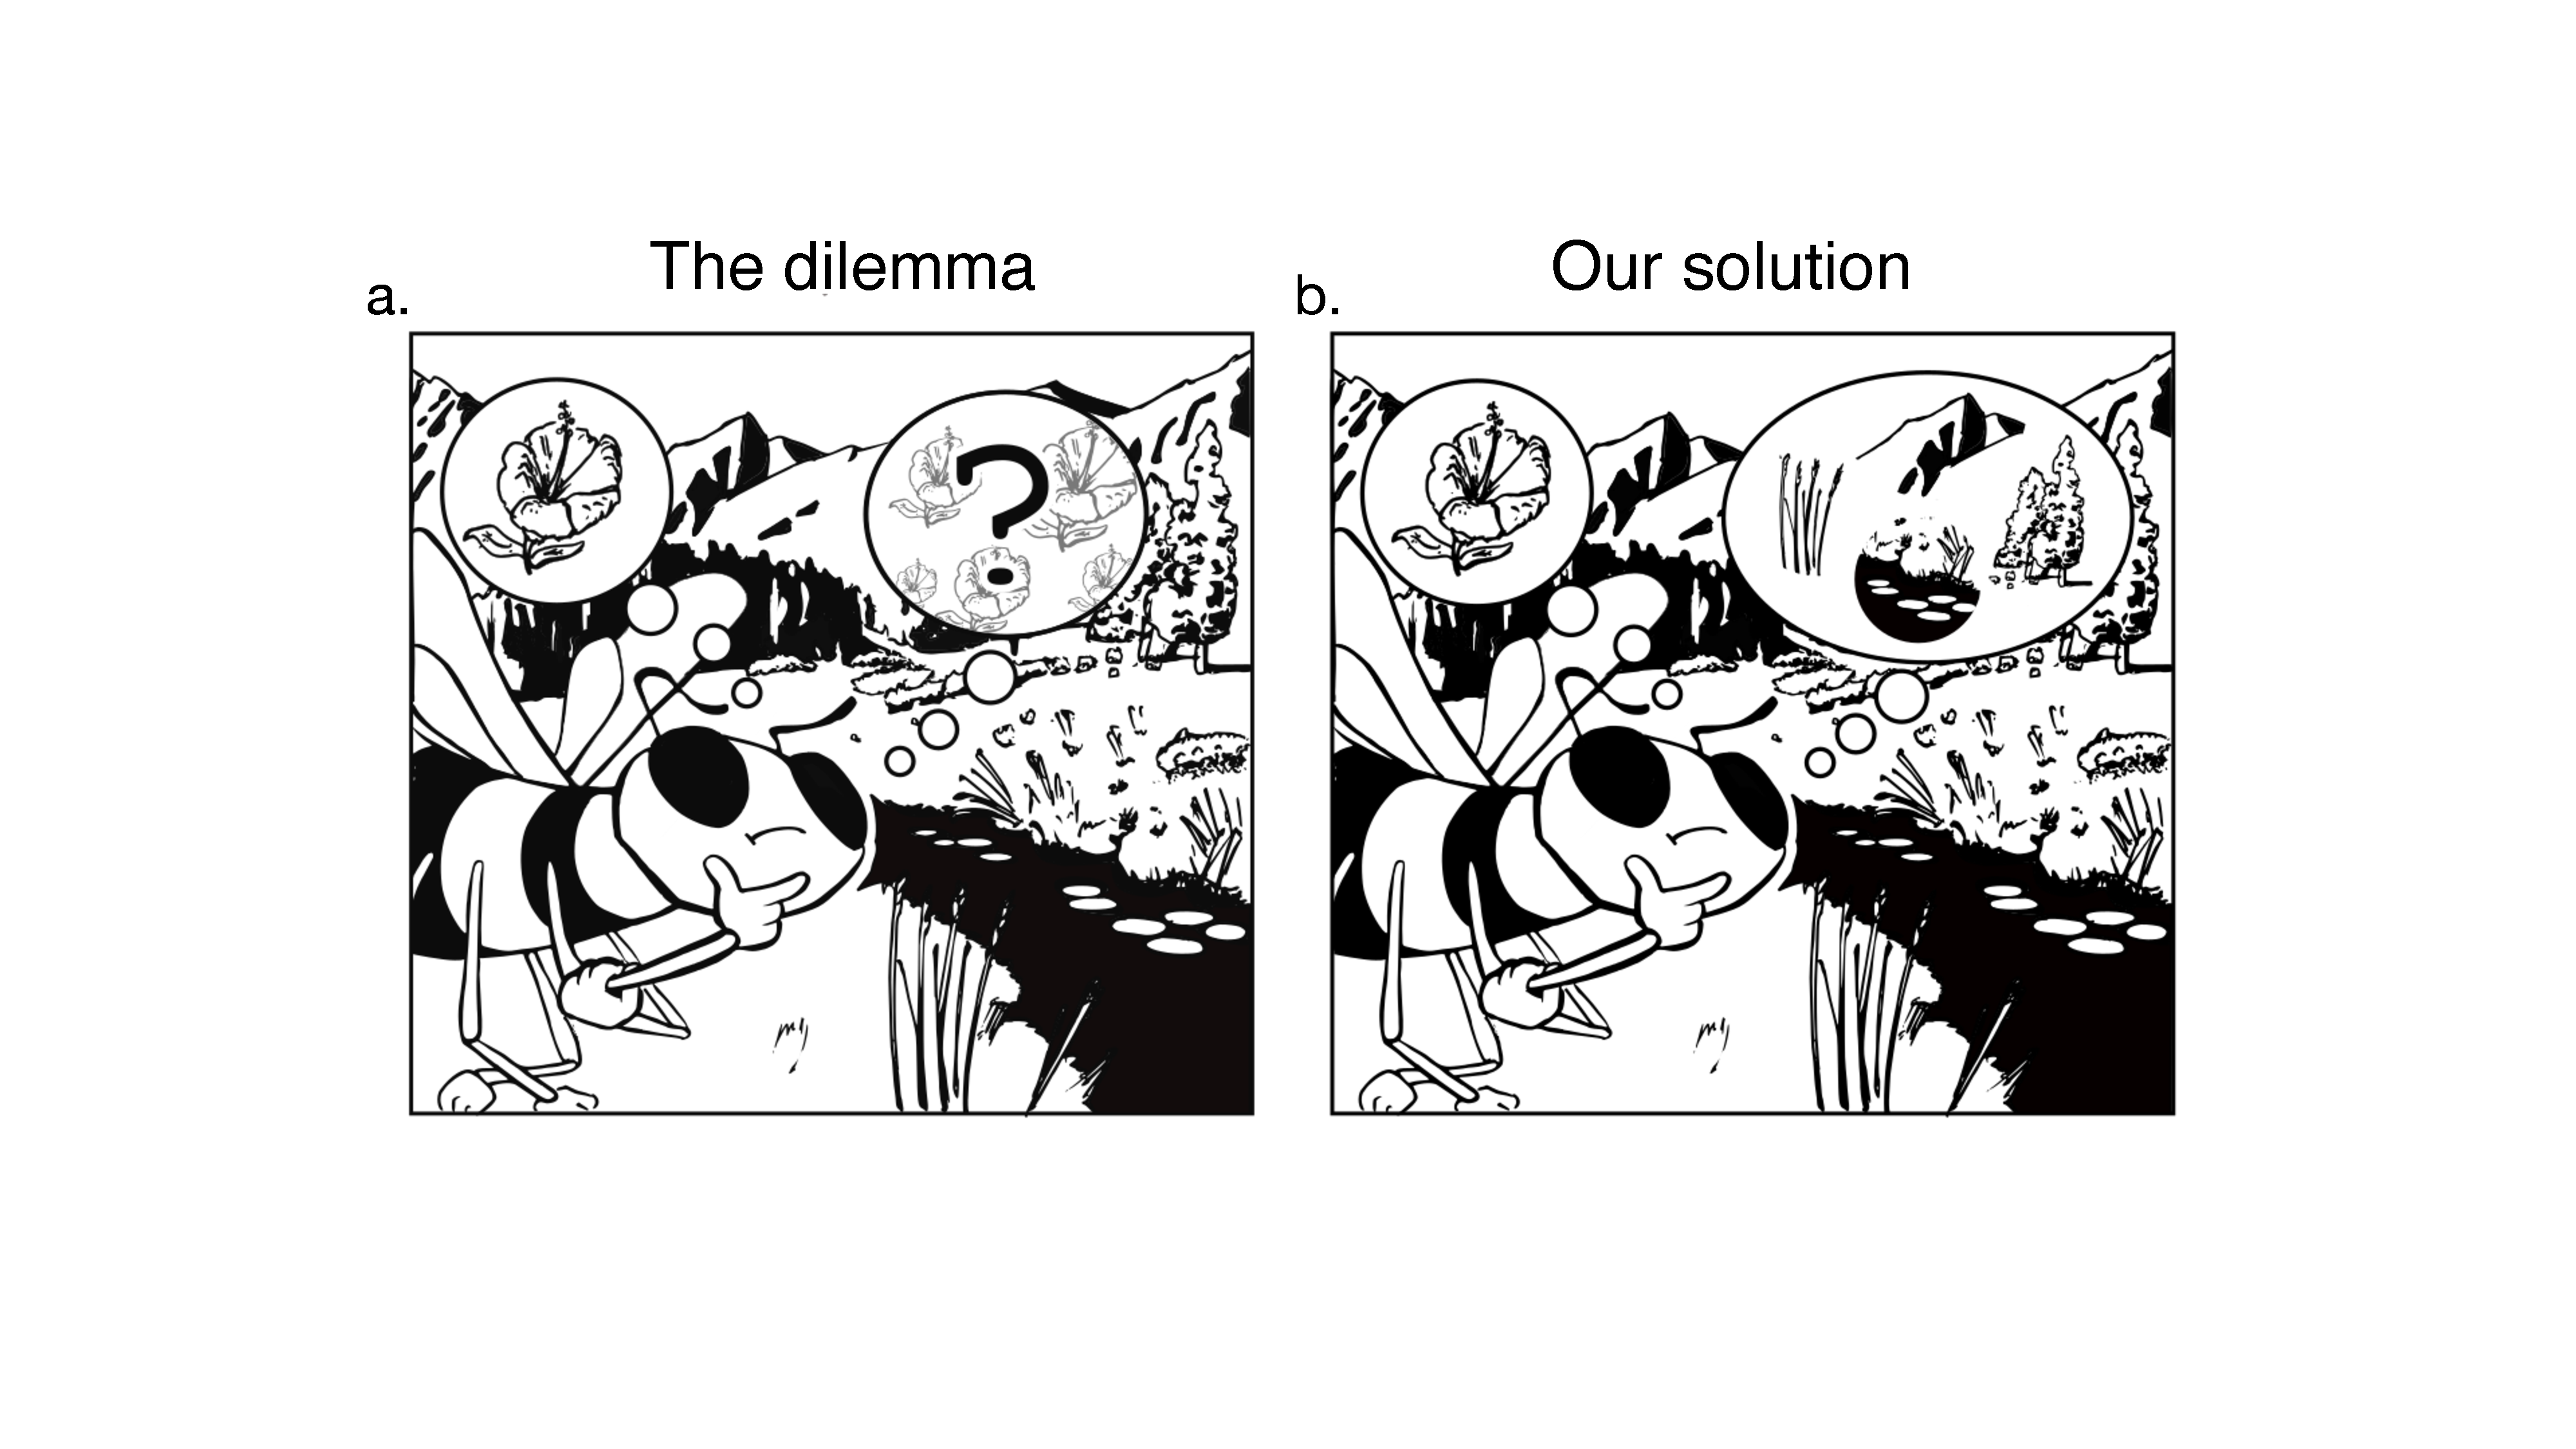
\includegraphics[width=.9\linewidth]{img/bee.pdf} 
	\caption{Two views of exploration and exploitation. \textbf{a}. The dilemma: either exploit an action with a known reward (e.g., return to the previous flower) or explore other actions on the chance they will return a better outcome. The central challenge here is that the outcome of exploration is uncertain, and filled with questions. \textbf{b}. An alternative view of the dilemma, with two goals: either maximize rewards \textit{or} maximize information value,s with a curious search of the environment. \textit{Artist credit}: Richard Grant.}
	\label{fig:bee} 
	\end{fullwidth}
\end{figure}

The first half of this paper we develop a the theory behind our union. This consists of mathmatical study of curiosity alone, and our mathematical solution to unifying curious with reward collection. The sescond half consists of some initial simulations. We demonstrtate exploration-out-of-curiosity leads to performance that is as good, if not better, than more standard approaches to the explore-exploit problems. We conclude with a some questions and answers about our approach.